\documentclass[11pt]{beamer} % mathserif for normal math fonts.
\usefonttheme[onlymath]{serif}
\usepackage[utf8]{inputenc}
\usepackage[swedish,english]{babel}
\usepackage{microtype}
\usepackage{amsmath,mathtools}
\usepackage{calc}
\usepackage{amsmath,mathtools,dsfont}
\usepackage{siunitx}
%\usepackage{movie15}
\usepackage{multimedia}
\usepackage{tikz}
\usepackage{pgfplots}
\usepackage{biblatex}
\usepackage{contmech}
\usepackage{grffile}
\usepackage{subfig}

\usepgfplotslibrary{patchplots}
\usepgfplotslibrary{groupplots}
\pgfplotsset{compat=1.3}

\DeclarePairedDelimiter{\homogenized}{\langle}{\rangle}
\newcommand{\pore}{\mathrm{p}}
\newcommand{\fluid}{\mathrm{f}}
\newcommand{\free}{\mathrm{f}}
\newcommand{\prescribed}{\mathrm{p}}
\newcommand{\moving}{\mathrm{mov}}
\newcommand{\segment}{\mathrm{segm}}
\newcommand{\corner}{\mathrm{corn}}
\newcommand{\surf}{\mathrm{s}}
\newcommand{\mesh}{\mathcal{M}}
\newcommand{\dirac}{\delta}
\newcommand{\on}{\quad\text{ on }}
%\newcommand{\on}{\mid}
\newcommand{\surfdiff}{\tilde{\ts\nabla}}
\newcommand{\at}[2]{\left.#1\right|_{#2}}

\newcommand{\roughcite}[1]{\textsc{#1}}

\usetheme[titleflower=true]{chalmers}
\title{Multiscale Modeling of Sintering of Hardmetal}
\author[Mikael Öhman et al.]{Mikael Öhman\and Kenneth Runesson\and Fredrik Larsson}
\institute{Dept. of Applied Mechanics\\ Chalmers University of Technology}
\titlepageextra{Svenska Mekanikdagarna 2011, Chalmers, Göteborg}
\date{June 13--15 2011}
\footer{\insertshortauthor\ SMD 2011}
\titlepagelogofile{figures/Avancez_black}
%\date{SMD 2011, Chalmers, Göteborg, June 13--15 2011}

% Bibliography
%\bibliography{references_extended}

\begin{document}

\section{Title page}
\begin{frame}[plain]
 \titlepage
\end{frame}

\section{Outline}
\begin{frame}
 \frametitle{Outline}

\begin{itemize}
 \item Background --- Motivation
 %\item Surface tension
 %\item Sintering phenomena on mesoscale
 \item Remarks on constitutive modeling
 \item Surface tension
 \item Multiscale modeling
 \item FE-code OOFEM: Object Oriented Finite Element Method
 \item Conclusions --- Future work
\end{itemize}
\end{frame}

%%%%%%%%%%%%%%%%%%%%%%%%%%%%%%%%%%%%%%%%%%%%%%%%%%%%%%%%%%%%%%%%%%%%%%%%%%%%%%%%%%%%%%%%%%%%%%%%%%%
\section{Background}
% \begin{frame}
%  \frametitle{Project background and motivation}
%  \begin{itemize}
%   \item Complicated macroscopic constitutive models
%   \begin{itemize}
%     \item Many parameters, impossible to measure
%     \item Needs experimental calibration
%   \end{itemize}
%   \item Computational power increasing
%  \end{itemize}
% 
%  \roughcite{Mähler, Ekh \& Runesson (1999)}
% 
%  \roughcite{Svoboda \& Reidel  (1996)}
% \end{frame}

\subsection{Process}
\begin{frame}
 \frametitle{Background --- Sintering of hardmetal}

% The sintering phenomenon on the mesoscale is driven by surface tension on the melted binder, and
% the homogenized effect of the surface tension is the so-called sintering stress.
% From the macroscopic perspective, the specimen (green body) shrinks due to this volumetric sintering stress. In the case of inhomogeneous
% initial density in the green body, the sintering can result in unwanted final deformations.

 \begin{enumerate}
  %\item Mixture of WC and Co particles (micrometer size)
  \item WC-particles surrounded by Co-matrix (binder metal)
  %\item Heating and softening of binder
  \item Precompaction $\rightarrow$ initial porosity 20--40\%
  \item Heating $\rightarrow$ thermal expansion, sintering driven by surface tension in melted Co-porespace, i.e. ``liquid phase sintering''
  \item Vanishing final porosity (ideal state)
  
  %\item Melting binder

  %\item Bridging between particles
  %\item Particles aggregate
  %\item Compaction due to surface tension
 \end{enumerate}
\alert{Note: Inhomogeneous initial density may lead to defect product:\\ \textsuperscript{(i)}remaining porosity, \textsuperscript{(ii)}shape imperfection }
\begin{center}
 \begin{columns}
 \column{0.25\textwidth}\centering
 \begin{tikzpicture}
   \node at (0,0) {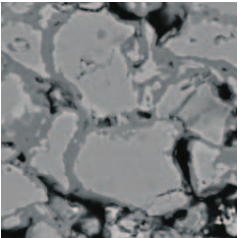
\includegraphics[width=\textwidth]{figures/sinter_1-crop.pdf}};
   \draw[red,thick,<-] (1,1) -- (1.5,1) node[right,black] {WC};
   \draw[red,thick,<-] (0.5,0.7) -- (1.5,0.5) node[right,black] {Co};
   \draw[red,thick,<-] (0.7,-0.3) -- (1.5,0) node[right,black] {pore};
 \end{tikzpicture}
 \column{0.05\textwidth}\centering
 $\xrightarrow{\text{idealized}}$
 \column{0.25\textwidth}\centering
 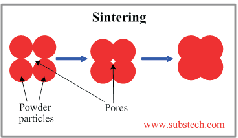
\includegraphics[width=\textwidth]{figures/sinter_2-crop.pdf}
 \end{columns}
 %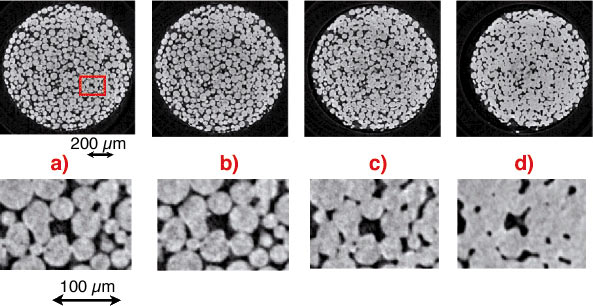
\includegraphics[width=0.6\textwidth]{figures/fig081.jpeg}
\end{center}
\end{frame}

%%%%%%%%%%%%%%%%%%%%%%%%%%%%%%%%%%%%%%%%%%%%%%%%%%%%%%%%%%%%%%%%%%%%%%%%%%%%%%%%%%%%%%%%%%%%%%%%%%%
\subsection{Comparison}
\begin{frame}
 \frametitle{Constitutive modeling}
 Macroscopic modeling of sintering
 \begin{itemize}
  \item Selected references: \roughcite{Svoboda \& Riedel (1996)}, \roughcite{Mähler, Ekh \& Runesson (1999)}
  \item Complex model structure, requires many parameters --- calibration problem very ill-posed
 \end{itemize}

 Multiscale modeling
 \begin{itemize}
  \item Selected references:  \roughcite{Geers \& coworkers (2001--)},
 \roughcite{Fish \& coworkers (1995--)},
 \roughcite{Miehe \& coworkers (2002--)},
 \roughcite{Larsson \& Runesson [adaptive multiscale] (2006--)}, \roughcite{Perić \& coworkers (2006)}
  \item Modeling of \textsuperscript{(i)}solid WC, \textsuperscript{(ii)}melt Co and \textsuperscript{(iii)}surface tension\\
  Note: Constitutive modeling refers to subscale constituents
  \item FE\textsuperscript{2} (FE on macro and mesoscales) based on computational homogenization on RVE:s
  \item Macroscale: Momentum balance
 \end{itemize}
\end{frame}

%%%%%%%%%%%%%%%%%%%%%%%%%%%%%%%%%%%%%%%%%%%%%%%%%%%%%%%%%%%%%%%%%%%%%%%%%%%%%%%%%%%%%%%%%%%%%%%%%%%
\section{Mesoscale}
\newcommand{\macroscale}{\mathrm{M}}
\newcommand{\subscale}{\mathrm{s}}
\begin{frame}
 \frametitle{RVE--problem: Viscous sintering}
 \begin{center}
  \begin{columns}
   \column{0.2\textwidth}
   \column{0.3\textwidth}\centering
    \resizebox{!}{0.8\textwidth}{\begin{tikzpicture}[>=latex,scale=2] % Use this to scale the image. Text is always normal-size
  \def\particleradius{1.05} % Adjust this to change the contact size.
  \pgfmathsetmacro{\contactsize}{sqrt(\particleradius^2-1)} % Automatically calculated.
  \begin{scope}[very thick]
  	\draw[clip] (-1,-1) rectangle (1,1);
  	\draw[clip]
  		(-1,-1) circle (\particleradius)
 		( 1,-1) circle (\particleradius)
 		(-1, 1) circle (\particleradius)
   		( 1, 1) circle (\particleradius);
  	\fill[fill=black!10] (-1,-1) rectangle (1,1);
  \end{scope}
  % Markers
  \foreach \q in {0,90,180,270} { \draw[rotate=\q] (1-\contactsize,-0.05) -- +(0,0.1); }
  \draw[dashed,gray] (-1.1,0) -- (1.1,0) (0,-1.1) -- (0,1.1);
  % Annotations
  %\node[below] at (0,0) {$\Omega_\Box^p(0)$};
  \draw[|<->|] (-1,-1.4) -- (1,-1.4) node[midway,above] {$L_\Box(0)$};
  \draw[<->|] (-1,-0.05) -- +(\contactsize,0) node[midway,below] {$a_0$};
  \node at (0.6,-0.6) {$\Omega_\Box^{\mathrm{part}}(0)$};
  \draw[<-] (1,-0.5) -- +(0.2,0) node[right] {$\Gamma_\Box(0)$};
  \draw[<-] (1,1) ++(-135:\particleradius) -- +(0.00,0.15) node[above right] {$\Gamma_\Box^{\mathrm{pore}}(0)$};
  
  %\draw[use as bounding box] (-1.7,-1.5) rectangle (1.7,1.1);
  %\useasboundingbox (-1.7,-1.5) (1.7,1.1);
  % Transformation arrow (makes the picture very unaligned)
  %\draw[->] (1.5,0) to[out=45,in=-150] (2,0);% +(135:0.1) -- (2,0) -- +(-135:0.1);
\end{tikzpicture}
}
   \column{0.3\textwidth}\centering
    \resizebox{!}{0.8\textwidth}{\begin{tikzpicture}[>=latex,scale=1.6] % Use this to scale the image. Text is always normal-size
  \def\particleradius{1.05} % Adjust this to change the contact size.
  \draw[thick,fill=black!10,even odd rule] (0.9,-1.1) 
  	to[out=190,in=10] (-1.1,-0.9)
  	to[out=80,in=-110] (-0.9,1.1)
  	to[out=10,in=-160] (1.1,1.1)
  	to[out=-100,in=60] (0.9,-1.1) -- cycle
  	(-0.1,-0.5) to[out=180,in=-45] (-0.2,-0.15) to[out=135,in=-90]
  	(-0.5,0)    to[out=90,in=-135] (-0.15,0.15)  to[out=45,in=-180]  
  	(0.1,0.5)   to[out=0,in=135]   (0.2,0.15)   to[out=-45,in=90] coordinate[near start] (GammaF)
  	(0.5,0)     to[out=-90,in=45]  (0.15,-0.15)  to[out=-135,in=0] (-0.1,-0.5) -- cycle;
  % Markers
  \draw[dashed,gray] (-1.1,0) to[out=5,in=-175] (1.1,0) (-0.2,-1.1) -- (0.2,1.1);
  % Annotations
  \node at (0.5,-0.6) {$\Omega_\Box(t)$};
  \draw[<-] (GammaF) -- +(0.00,0.15) node[above right] {$\Gamma_\Box^{\mathrm{pore}}(t)$};
\end{tikzpicture}}
   \column{0.2\textwidth}
  \end{columns}
 \end{center}
 \begin{itemize}
  \item Suface-tension driven microflow of single unit cell RVE
  \item RVE-problem with Dirichlet b.c. ``driven'' by macroscale rate-of-deformation $\bar{\ts d}\rightarrow$ subscale velocity:
	$\ts v = \ts v^\macroscale(\bar{\ts d})+\ts v^\subscale$

 For given $\bar{\ts d}$, solve for $\ts v^\subscale \in \mathds{V}_\square^{\mathrm{D}}, p \in \mathds{P}_\square$:
 \begin{align*}
  a_\square(\ts v^\macroscale(\bar{\ts d})+\ts v^\subscale; \delta\ts v^\subscale) + b_\square(p,\delta \ts v^\subscale) &= l_\square(\delta \ts v^\subscale)\quad &&\forall \delta \ts v^\subscale \in \mathds{V}_\square^{(\mathrm{D})},\\
 b_\square(\delta p,\ts v^\macroscale(\bar{\ts d}) + \ts v^\subscale) &= 0 && \forall \delta p\in \mathds P_\square.
 \end{align*}

 $l_\square(\delta \ts v^\subscale)$: loading by surface tension tractions on $\Gamma_\square^{\text{pore}}$
 \end{itemize}
\end{frame}

%%%%%%%%%%%%%%%%%%%%%%%%%%%%%%%%%%%%%%%%%%%%%%%%%%%%%%%%%%%%%%%%%%%%%%%%%%%%%%%%%%%%%%%%%%%%%%%%%%%
\subsection{Surface Tension}
\begin{frame}
 \frametitle{RVE-problem: Modeling of surface tension}
 Surface tension is modeled by a constant energy $\gamma_\surf$ per unit current area
\begin{gather*}
 \Psi_\surf = \int_{\Gamma_\Box^\free} \gamma_\surf \dif A = \int_{\Gamma_{\Box,0}^\free} \gamma_\surf \tilde J \dif A_0
\intertext{and the material derivative}
 \dot\Psi_\surf = \int_{\Gamma_{\Box,0}^\free} \gamma_\surf  \od{\tilde J}{t} \dif A_0
     = \int_{\Gamma_{\Box,0}^\free} \gamma_\surf \ta v\cdot\tilde\diff \tilde J \dif A_0
     = \int_{\Gamma_{\Box}^\free} \gamma_\surf \ta v\cdot\tilde\diff \dif A
\intertext{where the surface divergence is introduced}
  \tilde\diff \defeq (\ts I - \ta n\outerp\ta n)\cdot \diff
\end{gather*}
\end{frame}

%%%%%%%%%%%%%%%%%%%%%%%%%%%%%%%%%%%%%%%%%%%%%%%%%%%%%%%%%%%%%%%%%%%%%%%%%%%%%%%%%%%%%%%%%%%%%%%%%%%
\begin{frame}
 \frametitle{RVE-problem: Modeling of surface tension}
 For viscous flow we get the dissipation from the momentum balance
\begin{gather*}
 \Dissipation = \int_{\Omega_\Box} \ts\sigma\dprod (\ta v\outerp\diff)^\sym\dif V
\end{gather*}
Setting up the total free energy and its variation
\begin{gather*}
 \dot\Pi = \dot\Psi_\surf + \Dissipation\\
 \delta\dot\Pi = \delta\dot\Psi_\surf + \delta\Dissipation = 0
\end{gather*}
which leads to the weak form of the problem
\begin{gather*}
 \int_{\Omega_\Box} \ts\sigma\dprod(\delta\ta v \otimes \diff)^\sym \dif V = \int_{\Gamma_\Box^\free} \gamma_\surf \delta\ta v \cdot\tilde\diff \dif A
\label{eq:weak_form}
\end{gather*}
\end{frame}

%%%%%%%%%%%%%%%%%%%%%%%%%%%%%%%%%%%%%%%%%%%%%%%%%%%%%%%%%%%%%%%%%%%%%%%%%%%%%%%%%%%%%%%%%%%%%%%%%%%
\begin{frame}
 \frametitle{RVE-problem: Strong form}
 Using the surface divergence theorem %\cite{Steinmann2008:boundaryenergies}
 the integrals can be rewritten as
\begin{multline*}
 \int_{\Omega_\Box} (\ts\sigma\cdot\diff)\cdot \delta\ta v \dif V =
  -\int_{\Gamma_\Box^\free} (\ts\sigma\cdot\ta n)\cdot\delta\ta v\dif A\\
  -\int_{\Gamma_\Box^\free} \gamma_\surf H \ta n \cdot \delta\ta v \dif A
  +\int_{\partial\Gamma_\Box^\free} \gamma_\surf \ta m\cdot \delta\ta v \dif S
\end{multline*}
where $H\defeq \ta n \cdot \tilde\diff$ is the curvature.
This leads to the strong form
\begin{gather*}
 \ts\sigma\cdot\diff = \ts 0 \on \Omega_\Box\\
 \ts\sigma\cdot\ta n = -\gamma_\surf H \ta n \on \Gamma_{\Box,\mathrm{smooth}}^\free\\
 \ts\sigma\cdot\ta n_i = \dirac(\partial\Gamma_\Box^\free)\gamma_{\surf,i} \ta m_i \on \partial\Gamma_{\Box}^\free \label{eq:singular}
\end{gather*}
\roughcite{Steinmann \& coworkers (2009--)}, \, \roughcite{Perić \& coworkers (2006)}
\end{frame}

%%%%%%%%%%%%%%%%%%%%%%%%%%%%%%%%%%%%%%%%%%%%%%%%%%%%%%%%%%%%%%%%%%%%%%%%%%%%%%%%%%%%%%%%%%%%%%%%%%%
% \begin{frame}
%  \frametitle{RVE-problem: Modeling of surface tension}
%  \begin{itemize}
%   \item Traction from curvature of free surfaces
%  \begin{gather*}
%   \ta t = 2\kappa\gamma \ta n
% \end{gather*}
%  \item Weak form (based on surface-divergence theorem)
% \begin{gather*}
%  \gamma\int_\Omega 2 \kappa \ta w\cdot \ta n\dif A = \gamma\int_{\partial\Omega} \ta w\cdot\ta m\dif S - \gamma\int_\Omega \ts\nabla_s \cdot \ta w \dif A
%  \label{eq:curvature}
% \end{gather*}
%  \roughcite{Steinmann \& Javili (2008--)}
%  \item \alert{Note: Geometry dependent!} Possible to compute a tangent for higher order approximation
% 
%  \item Difficult/Costly to express load in Backward Euler scheme due to topological changes of merging surfaces
% 
%  \roughcite{Perić \& Coworkers (2006)}
%  \end{itemize}
% \end{frame}

\begin{frame}
 \frametitle{Mesoscale modeling of sintering}

 \begin{itemize}
  \item Incompressible Stokes flow problem
  \item Subscale FE-approximation
  \begin{itemize}
    \item Taylor-Hood element (quadratic $\ta v$, linear $p$)
    \item Surface tension element
  \end{itemize}
  \item Explicit time stepping
  \item Updated Lagrangian formulation
  %\item Simple constitutive driver
  \item \alert{Note: Finite macroscale compressibility despite incompressible subscale flow}
 \end{itemize}

\begin{figure}[hbpt]
 \centering
% Code to actually plot it.
%  \begin{tikzpicture}
%   \begin{groupplot}[
%     group style={group size=3 by 1},
%     width=4cm,
%     height=4cm,
%     xticklabels={},
%     yticklabels={},
%     %colormap/cool,
%     patch to triangles,
%     %patch refines=1,
% 	%shader=interp,
% 	%shader=flat,
%     %colorbar style={y=Pressure,title=Colorbar},
%    point meta min={-1.6}, % Had to look them manually. Might be possible to fetch from the first plot though.
%    point meta max={1.16}
%    ]
%   \nextgroupplot
%   \addplot[patch,patch table={figures/connectivity_tri2.dat},patch type=triangle quadr, ultra thin, point meta=\thisrow{p}]
%     table[x=x,y=y] {figures/nodes_1.dat};
%   \addplot[patch,mesh,patch table={figures/connectivity_edge.dat},patch type=quadratic spline, thick, draw=black]
%     table[x=x,y=y] {figures/nodes_1.dat};
%   \nextgroupplot%[xtick=\emtpy]
%   \addplot[patch,patch table={figures/connectivity_tri2.dat},patch type=triangle quadr, ultra thin, point meta=\thisrow{p}]
%     table[x=x,y=y] {figures/nodes_50.dat};
%   \addplot[patch,mesh,patch table={figures/connectivity_edge.dat},patch type=quadratic spline, thick, draw=black]
%     table[x=x,y=y] {figures/nodes_50.dat};
%   \nextgroupplot%[colorbar,colorbar right, colorbar style={ylabel=Pressure}]
%   \addplot[patch,patch table={figures/connectivity_tri2.dat},patch type=triangle quadr, ultra thin, point meta=\thisrow{p}]
%     table[x=x,y=y] {figures/nodes_200.dat};
%   \addplot[patch,mesh,patch table={figures/connectivity_edge.dat},patch type=quadratic spline, thick, draw=black]
%     table[x=x,y=y] {figures/nodes_200.dat};
%   \end{groupplot}
%   \draw[thick,black,->,shorten >=5pt,shorten <=5pt] (group c1r1.east) -- (group c2r1.west);
%   \draw[thick,black,->,shorten >=5pt,shorten <=5pt] (group c2r1.east) -- (group c3r1.west);
%  \end{tikzpicture}
 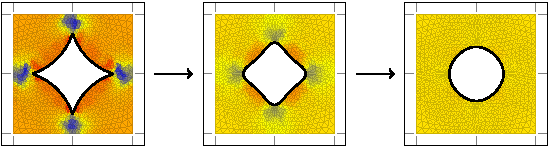
\includegraphics{figures/rve_evolve.pdf} % Manually externalized it
 \caption{Evolution of free surface within an RVE}\label{fig:rve_evolution}
\end{figure}
\end{frame}

%%%%%%%%%%%%%%%%%%%%%%%%%%%%%%%%%%%%%%%%%%%%%%%%%%%%%%%%%%%%%%%%%%%%%%%%%%%%%%%%%%%%%%%%%%%%%%%%%%%
\subsection{Results}
% \begin{frame}
%  \frametitle{Numerical results: Single RVE}
% \begin{center}
% \movie[height=6cm,width=6cm,poster]{
\includegraphics[width=5cm]{figures/free_1x1.0000}}{RVE_Fixed_Boundaries.avi}
% 
% \movie[externalviewer]{RVE with fixed boundaries --- macroscopically rigid}{RVE_Fixed_Boundaries.avi}
% \end{center}
% \end{frame}

%%%%%%%%%%%%%%%%%%%%%%%%%%%%%%%%%%%%%%%%%%%%%%%%%%%%%%%%%%%%%%%%%%%%%%%%%%%%%%%%%%%%%%%%%%%%%%%%%%%
\begin{frame}
 \frametitle{Numerical results: Single RVE}
\vspace{-1em}
\begin{figure}[thpb!]
    \centering
    \subfloat[$t = 0$]{
\includegraphics[width=0.2\linewidth]{figures/evolve_fixed_1}\label{fig:evolve_fixed_a}}
    \hspace{0.3em}
    \subfloat[$t = \frac12 t_{\mathrm{end}}$]{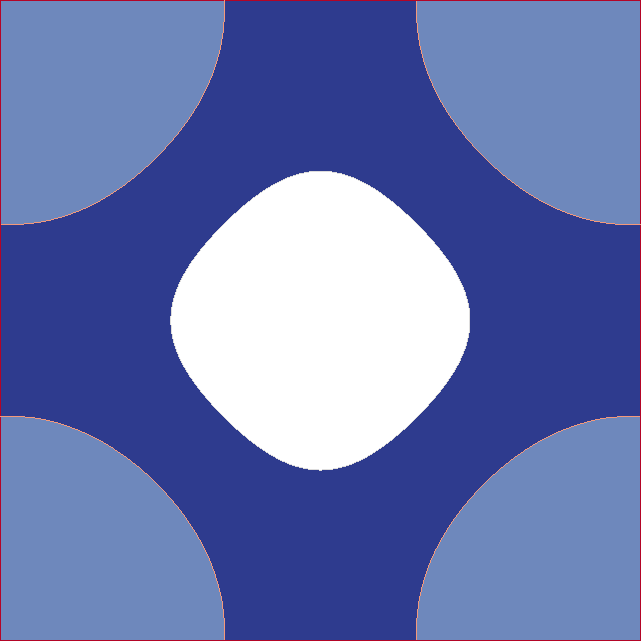
\includegraphics[width=0.2\linewidth]{figures/evolve_fixed_250}\label{fig:evolve_fixed_b}}
    \hspace{0.3em}
    \subfloat[$t = t_{\mathrm{end}}$]{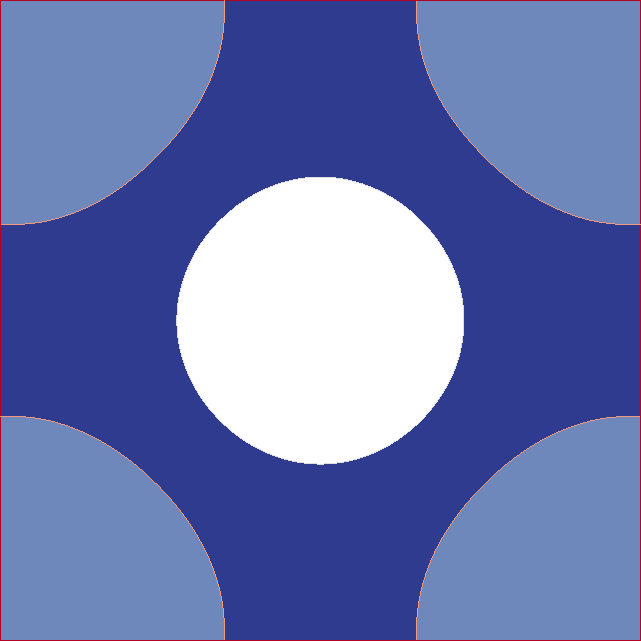
\includegraphics[width=0.2\linewidth]{figures/evolve_fixed_500}\label{fig:evolve_fixed_c}}
    \caption{Snapshots of computed RVE-configurations at selected times. Subject to fixed boundaries: $\bar{\ts d}= \ts 0$}
    \label{fig:fixed}
\end{figure}
\vspace{-1.5em}
\begin{figure}[thpb!]
  \centering
  \begin{tikzpicture}
  \begin{axis}[ xtick={0,0.2,...,1},
                tick label style={font=\scriptsize},
                height=0.25\textwidth, width=0.7\textwidth, xmin=0, xmax=1, ymax=0,
                xlabel={\small$t/t_{\mathrm{end}}$}, ylabel={\small$\bar\sigma_\mean/p_\nominal$}]
    \addplot[thick] file {figures/s_mean.txt};
    %\addplot[thick] file {figures/shear_s_mean.txt};
  \end{axis}
  \end{tikzpicture}
  \caption{Evolution of the normalized volumetric stress over time. Subject to fixed boundaries: $\bar{\ts d}= \ts 0$}
  \label{fig:fixed_graph}
\end{figure}

\end{frame}

%%%%%%%%%%%%%%%%%%%%%%%%%%%%%%%%%%%%%%%%%%%%%%%%%%%%%%%%%%%%%%%%%%%%%%%%%%%%%%%%%%%%%%%%%%%%%%%%%%%
\begin{frame}
 \frametitle{Numerical results: Single RVE}
\begin{center}
\movie[height=5cm,width=5cm,poster]{
\includegraphics[width=5cm]{figures/free_1x1.0000}}{free_1x1.wmv}
\movie[height=5cm,width=5cm,poster]{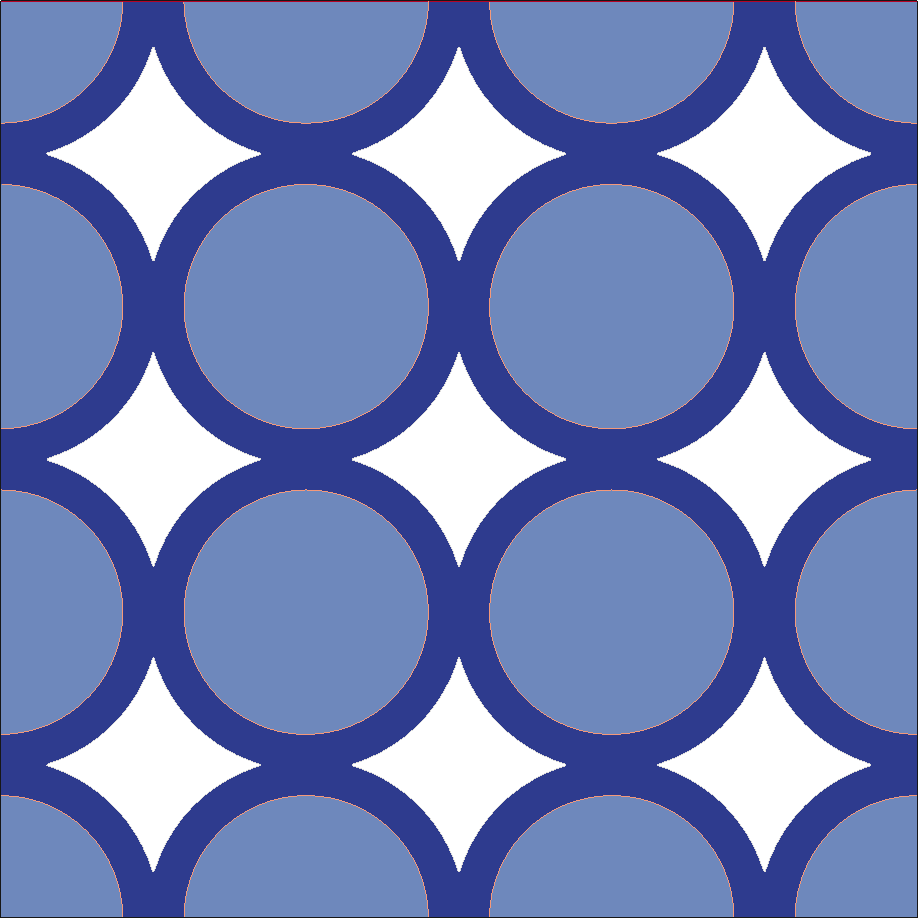
\includegraphics[width=5cm]{figures/free_3x3.0000}}{free_3x3.wmv}

\movie[externalviewer]{RVE with free Dirichlet boundaries -- macroscopically zero stress}{rve_3x3.wmv}
\end{center}
\end{frame}

%%%%%%%%%%%%%%%%%%%%%%%%%%%%%%%%%%%%%%%%%%%%%%%%%%%%%%%%%%%%%%%%%%%%%%%%%%%%%%%%%%%%%%%%%%%%%%%%%%%
\begin{frame}
 \frametitle{Numerical results: Single RVE}
\begin{figure}
 \centering
  \includegraphics[width=\linewidth]{figures/vs_densitet-crop}
 \caption{Evolution of the relative density}
\end{figure}

\end{frame}

%%%%%%%%%%%%%%%%%%%%%%%%%%%%%%%%%%%%%%%%%%%%%%%%%%%%%%%%%%%%%%%%%%%%%%%%%%%%%%%%%%%%%%%%%%%%%%%%%%%
\section{Macroscale}
\begin{frame}
 \frametitle{Multiscale implementation}
\begin{columns}
\column{0.51\textwidth}
 Subscale
 \begin{itemize}
  \item Dirichlet b.c. on RVE
  \item Very large deformations.
  \item Remeshing
  \item Explicit formulation
 \end{itemize}

 Macroscale
 \begin{itemize}
  \item Momentum balance with internal volumetric stress.
  \item \alert{Present limitation:} When pores vanish, RVE's become incompressible.
 \end{itemize}
\column{0.49\textwidth}

\begin{center}
 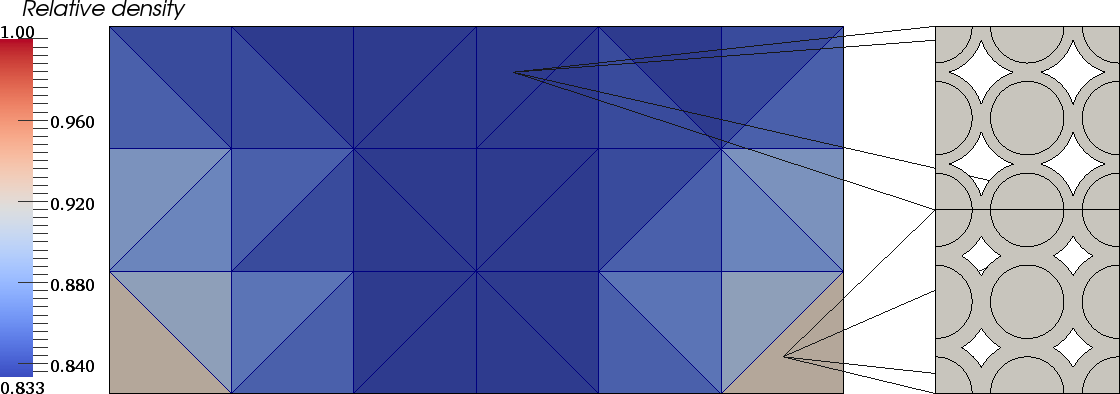
\includegraphics[width=0.9\linewidth]{figures/macro_sintering_2x2.0000}\\
 $\longrightarrow$\\[0.5em]
 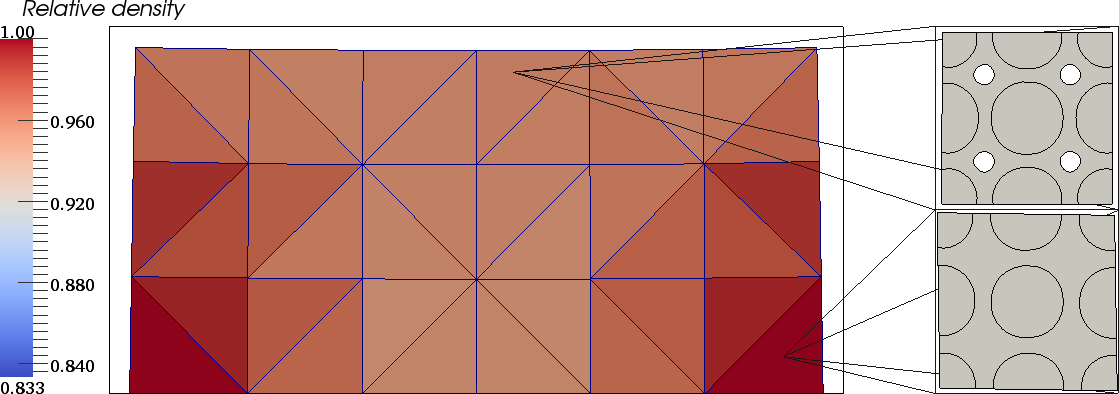
\includegraphics[width=0.9\linewidth]{figures/macro_sintering_2x2.0176}
\end{center}
\end{columns}
 \vspace{0.5em}
 Computational homogenization with Dirichlet boundary conditions.

\end{frame}

%%%%%%%%%%%%%%%%%%%%%%%%%%%%%%%%%%%%%%%%%%%%%%%%%%%%%%%%%%%%%%%%%%%%%%%%%%%%%%%%%%%%%%%%%%%%%%%%%%%
\subsection{Results}
\begin{frame}
 \frametitle{Numerical results}
\begin{center}
\movie[width=\linewidth]{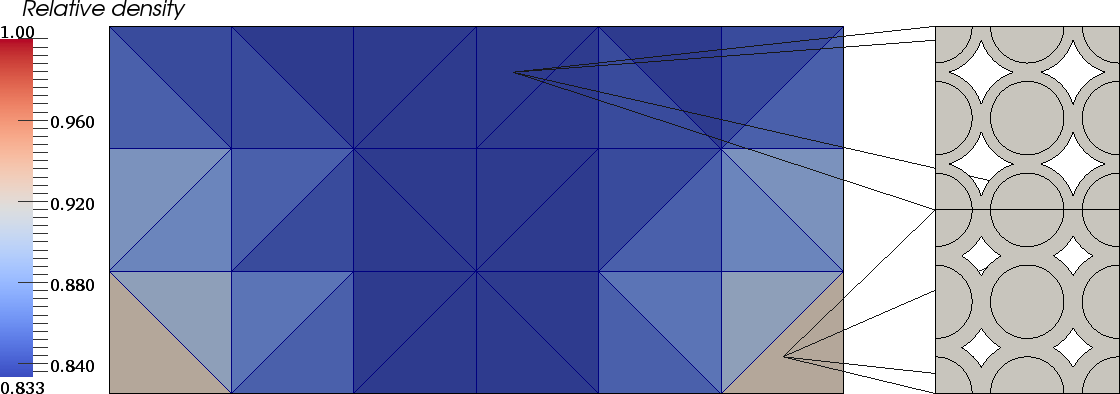
\includegraphics[width=\linewidth]{figures/macro_sintering_2x2.0000}}{macro_sintering_2x2.wmv}
%1120x394 movie
\movie[externalviewer]{Multiscale sintering}{Sintering_5x5.mpeg}
\end{center}
\end{frame}

%%%%%%%%%%%%%%%%%%%%%%%%%%%%%%%%%%%%%%%%%%%%%%%%%%%%%%%%%%%%%%%%%%%%%%%%%%%%%%%%%%%%%%%%%%%%%%%%%%%
\section{Implementation}
\subsection{OOFEM}
\begin{frame}
 \frametitle{OOFEM -- Finite element code}
\onslide<1-> Characteristics of OOFEM
 \begin{enumerate}
  \item<1-> Parallel computations: Designed for message passage paradigm
  \item<1-> Sparse matrix structures
  \item<1-> Nonlinear solvers
  \begin{itemize}
   \item<1-> Several linear solvers
   \item<1-> Line-search solvers
   \item<1-> Newton solvers
  \end{itemize}
  \item<1-> Interpolation and integration
  \item<1-> Exporting data
  \item<1-> Adaptivity
  \item<1-> Cooperation, \url{http://www.oofem.org/}
 \end{enumerate}

 \onslide<2-> Implementation
 \begin{enumerate}
  \item<2-> Subscale FE-problem replaces conventional constitutive model
  \item<2-> Complementing and extending existing code as needed
 \end{enumerate}

\end{frame}

%%%%%%%%%%%%%%%%%%%%%%%%%%%%%%%%%%%%%%%%%%%%%%%%%%%%%%%%%%%%%%%%%%%%%%%%%%%%%%%%%%%%%%%%%%%%%%%%%%%
\section{Conclusions --- Future}
\begin{frame}
 \frametitle{Conclusions --- Future work}
 So far
 \begin{enumerate}
  %\item Captures the most important properties of sintering with only two material parameters
  \item FE\textsuperscript{2} computational homogenization of subscale viscous flow driven by surface tension
  \item Clean, modular, implementation in OOFEM. Easy to extend.
  \item Surface tracking with remeshing, vanishing pores.
 \end{enumerate}

 Future work
 \begin{enumerate}
  \item Eventual macroscopic incomrpessibility $\implies$ mixed $(\bar{\ta v},\bar{p})$-format
  \item Statistical properties of microstructures
  \item 3D with realistic microstructural topology
  \item Weakly periodic boundary conditions (Neumann boundary condition as special case)
  \item Comparison with macroscopic experiments
 \end{enumerate}

\end{frame}

%%%%%%%%%%%%%%%%%%%%%%%%%%%%%%%%%%%%%%%%%%%%%%%%%%%%%%%%%%%%%%%%%%%%%%%%%%%%%%%%%%%%%%%%%%%%%%%%%%%

\end{document}
